\section{Print Controls}

\subsection{Approach}
There are many ways to create an FDM 3D printer, as seen in the many models available on the market, from industry-serving companies like Stratasys\footnote{\url{http://www.stratasys.com/}} and 3D Systems\footnote{\url{http://www.3dsystems.com/}} to home printer startups like Makerbot\footnote{\url{http://www.makerbot.com/}} to the many open-source efforts, notably the RepRap\footnote{\url{http://reprap.org/}} ecosystem. Most of these printers operate on Cartesian-style gantry system with 3 degrees of freedom. Some curved-layer printing is attainable on such printers, but the fixed attitude of the print heads limits the layer geometries to those that are accessible from one approach angle. To get around this limitation, a 6-degree-of-freedom robotic arm from FANUC\footnote{\url{http://www.fanucamerica.com/}} was used for this project. In addition to providing the 6 degrees of freedom necessary for curved-layer printing, the robot also provides 0.02mm of positioning repeatibility, which is small with respect to typical FDM nozzle outlet diameters (0.2-0.4mm). The robot was purchased in 2010 in the iRVision package as part of the CERT Program from FANUC. See the program brochure in Section~\ref{sec:cert-brochure} for more details.

Once the robot was chosen as the printing platform, much of the remaining 3D printing toolchain was filled in with parts and software from the RepRap community. These included the extruder hot-end and some related control hardware and software. Some additional control components were purchased from FANUC or fabricated in-house.

\subsection{Overview}
Figure~\ref{fig:sys-overview} gives a schematic overview of the mechanical, hardware, and software components that make up the curved-layer 3D printer system. The robot arm is the mechanical platform for the 3D printer. The custom extruder is fitted to the end of the robot arm and acts as a printing end effector. The motion of the robot arm is controlled by the robot controller, which is programmed by writing TP programs via the controller teach pendant. The extruder hardware, including the heater cartridge, cooling fan, and extrusion motor are controlled by an open-source Megatronics board loaded with the (also open-source) Marlin\footnote{\url{http://reprap.org/wiki/Marlin}} firmware. 

Normally, the Megatronics board is used to control the path of the extruder as well as the extrusion feed rate; the Marlin firmware can thus adjust the extruder filament feedrate according to the surface speed of the extruder in order to maintain the desired volumetric flow rate of hot plastic. However, in this case, the extruder path is controlled by the robot controller, so the extrusion control is independent of the motion control. Ideally, the two systems would be interfaced to allow the robot controller to give look-ahead speed predictions to the extruder controller to allow for tight synchronization. However, the FANUC controller interface only allows such interfacing with approved machinery. The next best option was to add I/O hardware to the FANUC controller and output an analog robot speed signal to the extruder controller. This way, the extruder controller might be able to extrude filament reasonably close to the actual extruder speed by tracking the robot speed output.

\begin{figure}
    \centering
    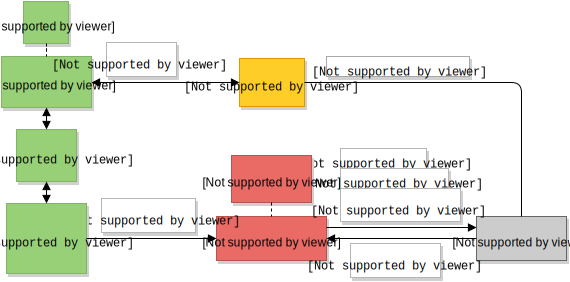
\includegraphics[width=.8\linewidth]{figures/diagrams/system overview}
    \caption{Overview of the 3D printer controls.}
    \label{fig:sys-overview}
\end{figure}

A more detailed electrical schematic is shown in Figure~\ref{fig:schem-fig}. 

\begin{figure}
    \centering
    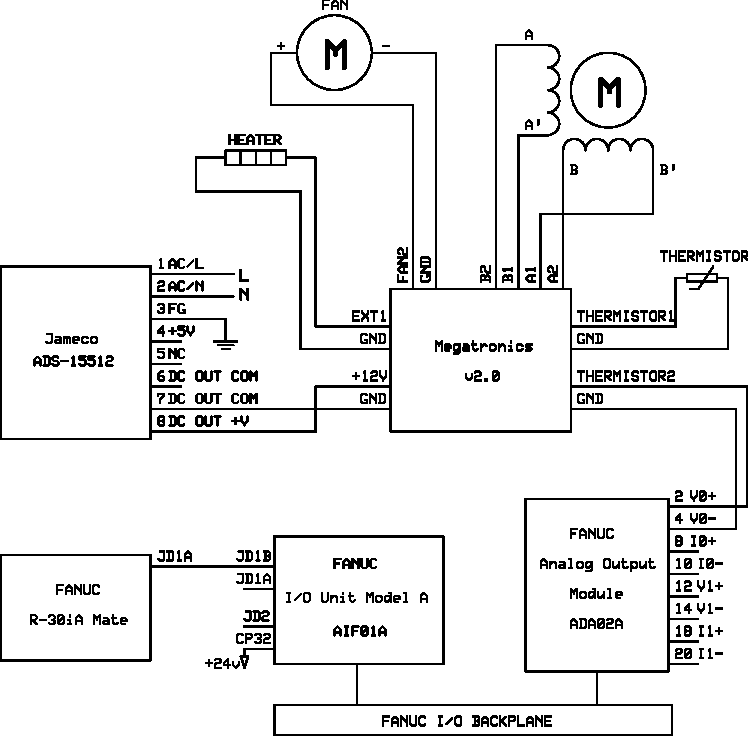
\includegraphics[width=.8\linewidth]{figures/diagrams/schematic-figure}
    \caption{Electrical schematic of the 3D printer controls.}
    \label{fig:schem-fig}
\end{figure}


\subsection{FANUC I/O interface}
\label{sec:io-interface}
The FANUC robot controller makes digital and analog electrical signals available to the user through the teach pendant interface \cite[sec~3.1.3]{lr-handling-tool}. However, in order to physically access these signals, additional I/O hardware is required. For this purpose, a FANUC backplane was purchased, as well as a corresponding I/O interface model and analog output module. Installation, maintenance, and usage information for these parts is available in \cite{io-unit}. The backplane and I/O interface module were purchased together as part of an I/O starter kit\footnote{from an eBay surplus seller.} for R-30iA controllers. The kit also included the I/O link cable, which connects the I/O interface unit to the controller and optional additional interface units; a grounding wire assembly for the backplane; and a male-male wire assembly for powering the I/O interface module. The analog output module was purchased separately. 

\subsubsection{Modules}
The I/O Unit Model A (interface module) makes the I/O points of the FANUC robot controller accessible through additional I/O modules. The interface module is installed in the first slot of the backplane, as shown in \cite[p~10]{io-unit}. The analog output module is installed in the next slot, and the remaining four slots are left empty.

\subsubsection{Wiring and connections}
The I/O interface module is connected to the controller and power supply according to \cite[ch~4]{io-unit}. In some configurations, the I/O interface unit would receive power from an auxiliary controller (a CNC machine, for instance) over the included cable. In this case, an external supply was needed. Additionally, the included grounding wire was too short to reach the inside of the existing FANUC controller from its desired location on the backplane. Thus, a power supply (CUI Inc EPS240025-P5P, datasheet in Section~\ref{sec:io-power}) and grounding wire were selected according to \cite[sec~4.2]{io-unit} and \cite[sec~4.3]{io-unit}, respectively. The power supply was spliced to the included power wire; the result is shown in Figure~\ref{fig:io-power}. Figures~\ref{fig:io-door} and \ref{fig:io-ground} show the I/O link cable connected on the back of the controller door and attached to the grounding plate as shown in \cite[Fig.3.2.2]{controller-maintenance}. Figure~\ref{fig:io-ground} also shows the installed ground wire for the I/O backplane, as described in \cite[sec~4.3]{io-unit}.

The analog output module offers two channels, each with a voltage output and a current output. The Channel 0 voltage output was chosen; the module pinout is available in \cite[sec~7.1.3]{io-unit}.

\begin{figure}
    \centering
    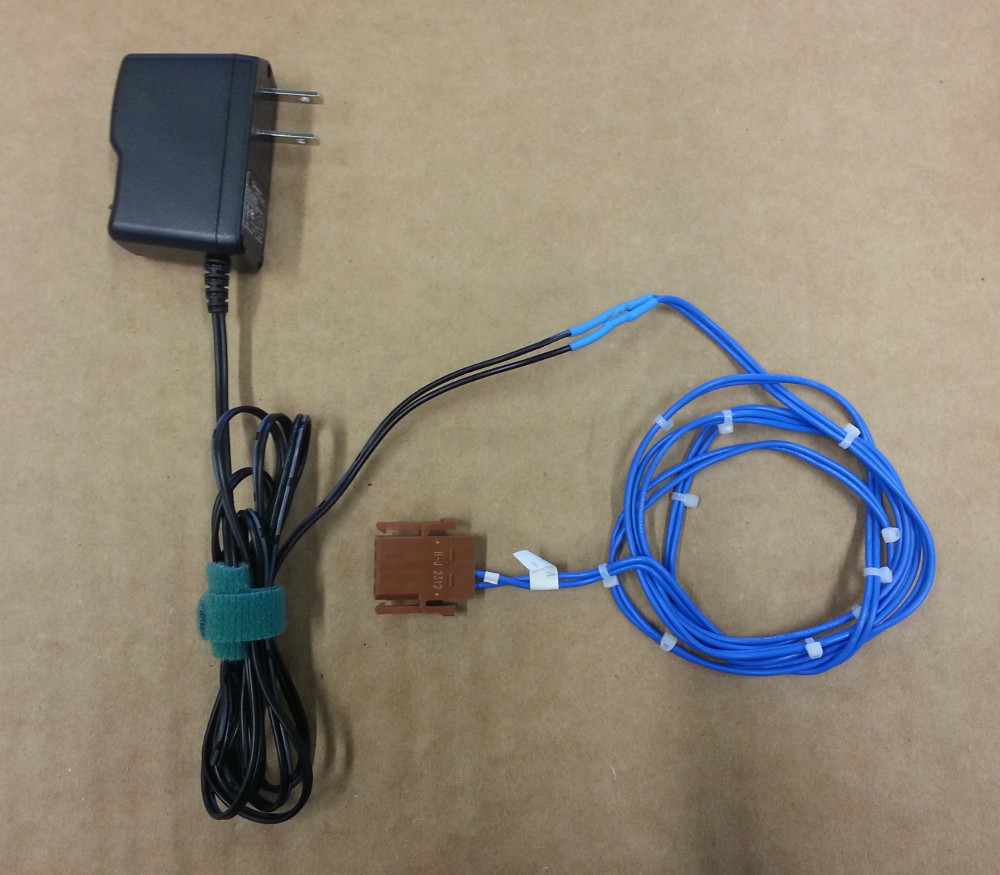
\includegraphics[width=.8\linewidth]{figures/io-power-splice}
    \caption{I/O interface module power supply.}
    \label{fig:io-power}
\end{figure}

\begin{figure}
    \centering
    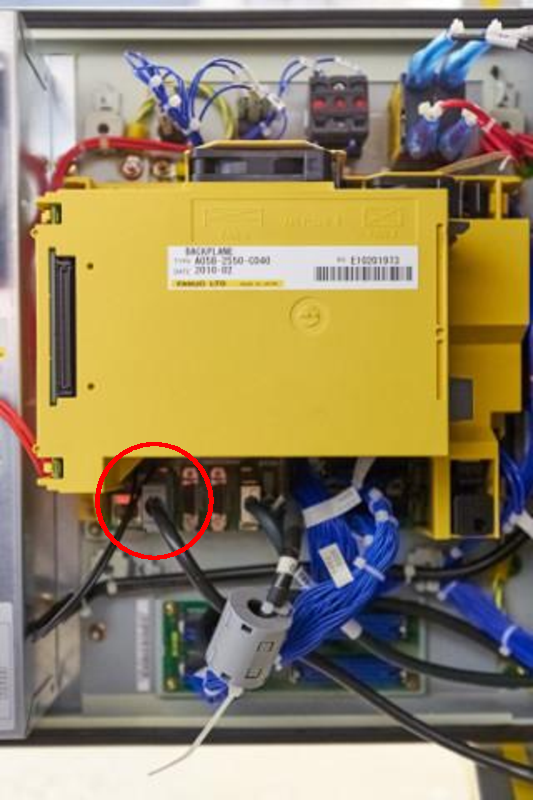
\includegraphics[width=.5\linewidth]{figures/diagrams/io-door-circled}
    \caption{I/O link cable installed in cabinet door.}
    \label{fig:io-door}
\end{figure}

\begin{figure}
    \centering
    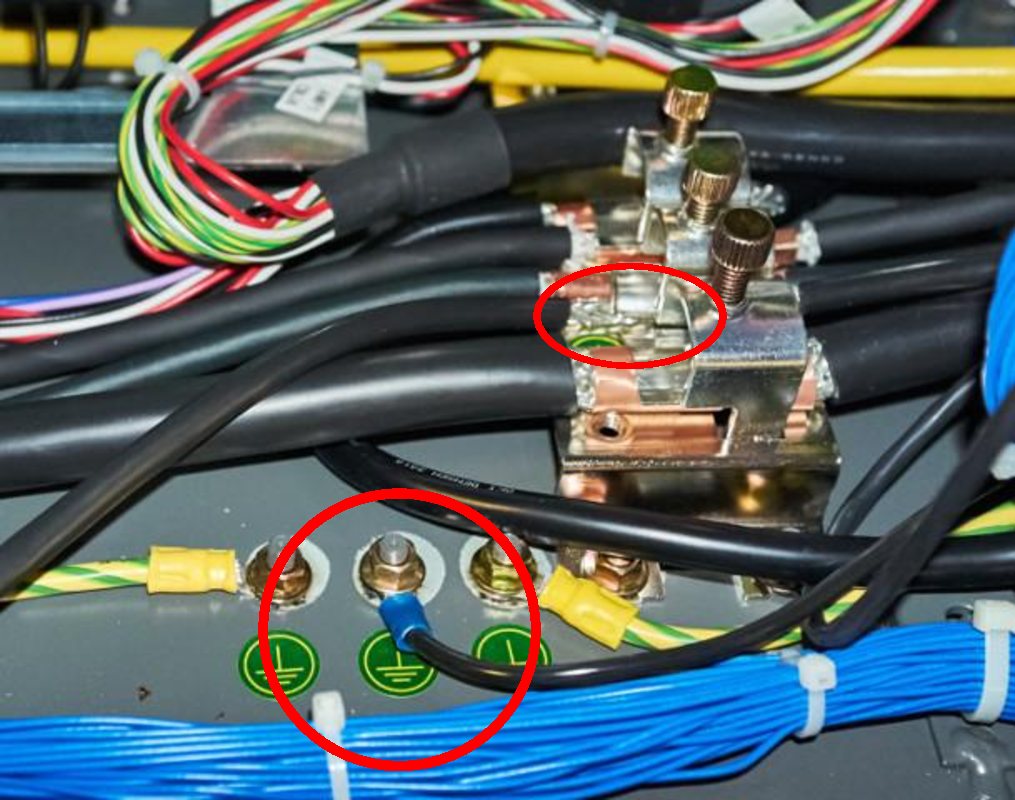
\includegraphics[width=.8\linewidth]{figures/diagrams/io-ground-circled}
    \caption{I/O link cable and back plane grounding.}
    \label{fig:io-ground}
\end{figure}

\subsubsection{Housing design}
A housing cabinet was designed and built to protect the I/O modules and allow access for maintenance and further expansion. The installed cabinet is shown in Figures~\ref{fig:cabinet1} and ~\ref{fig:cabinet2}. The cabinet was designed with inside dimensions according to \cite[sec~3.2]{io-unit}. Because the total heat generation of the two modules is only 4.3W, according to \cite[Table~3.3]{io-unit}, no special ventilation features were added. Clear polycarbonate was chosen as the cabinet material for easy visual checking of the I/O interface module status lights and proper wiring. The polycarbonate panels were adhered together with a SCIGRIP acrylic cement\footnote{\url{http://www.scigrip.com/product.php?id=16}}. The cabinet mounts to the CERT cart frame alongside the FANUC controller. Felt washers, shown in Figure~\ref{fig:felt-washer}, were used to protect the cabinet bottom from the frame members. Drawings and a bill of materials for the cabinet are available in Appendix~\ref{sec:cabinet-drawings}.

\begin{figure}
    \centering
    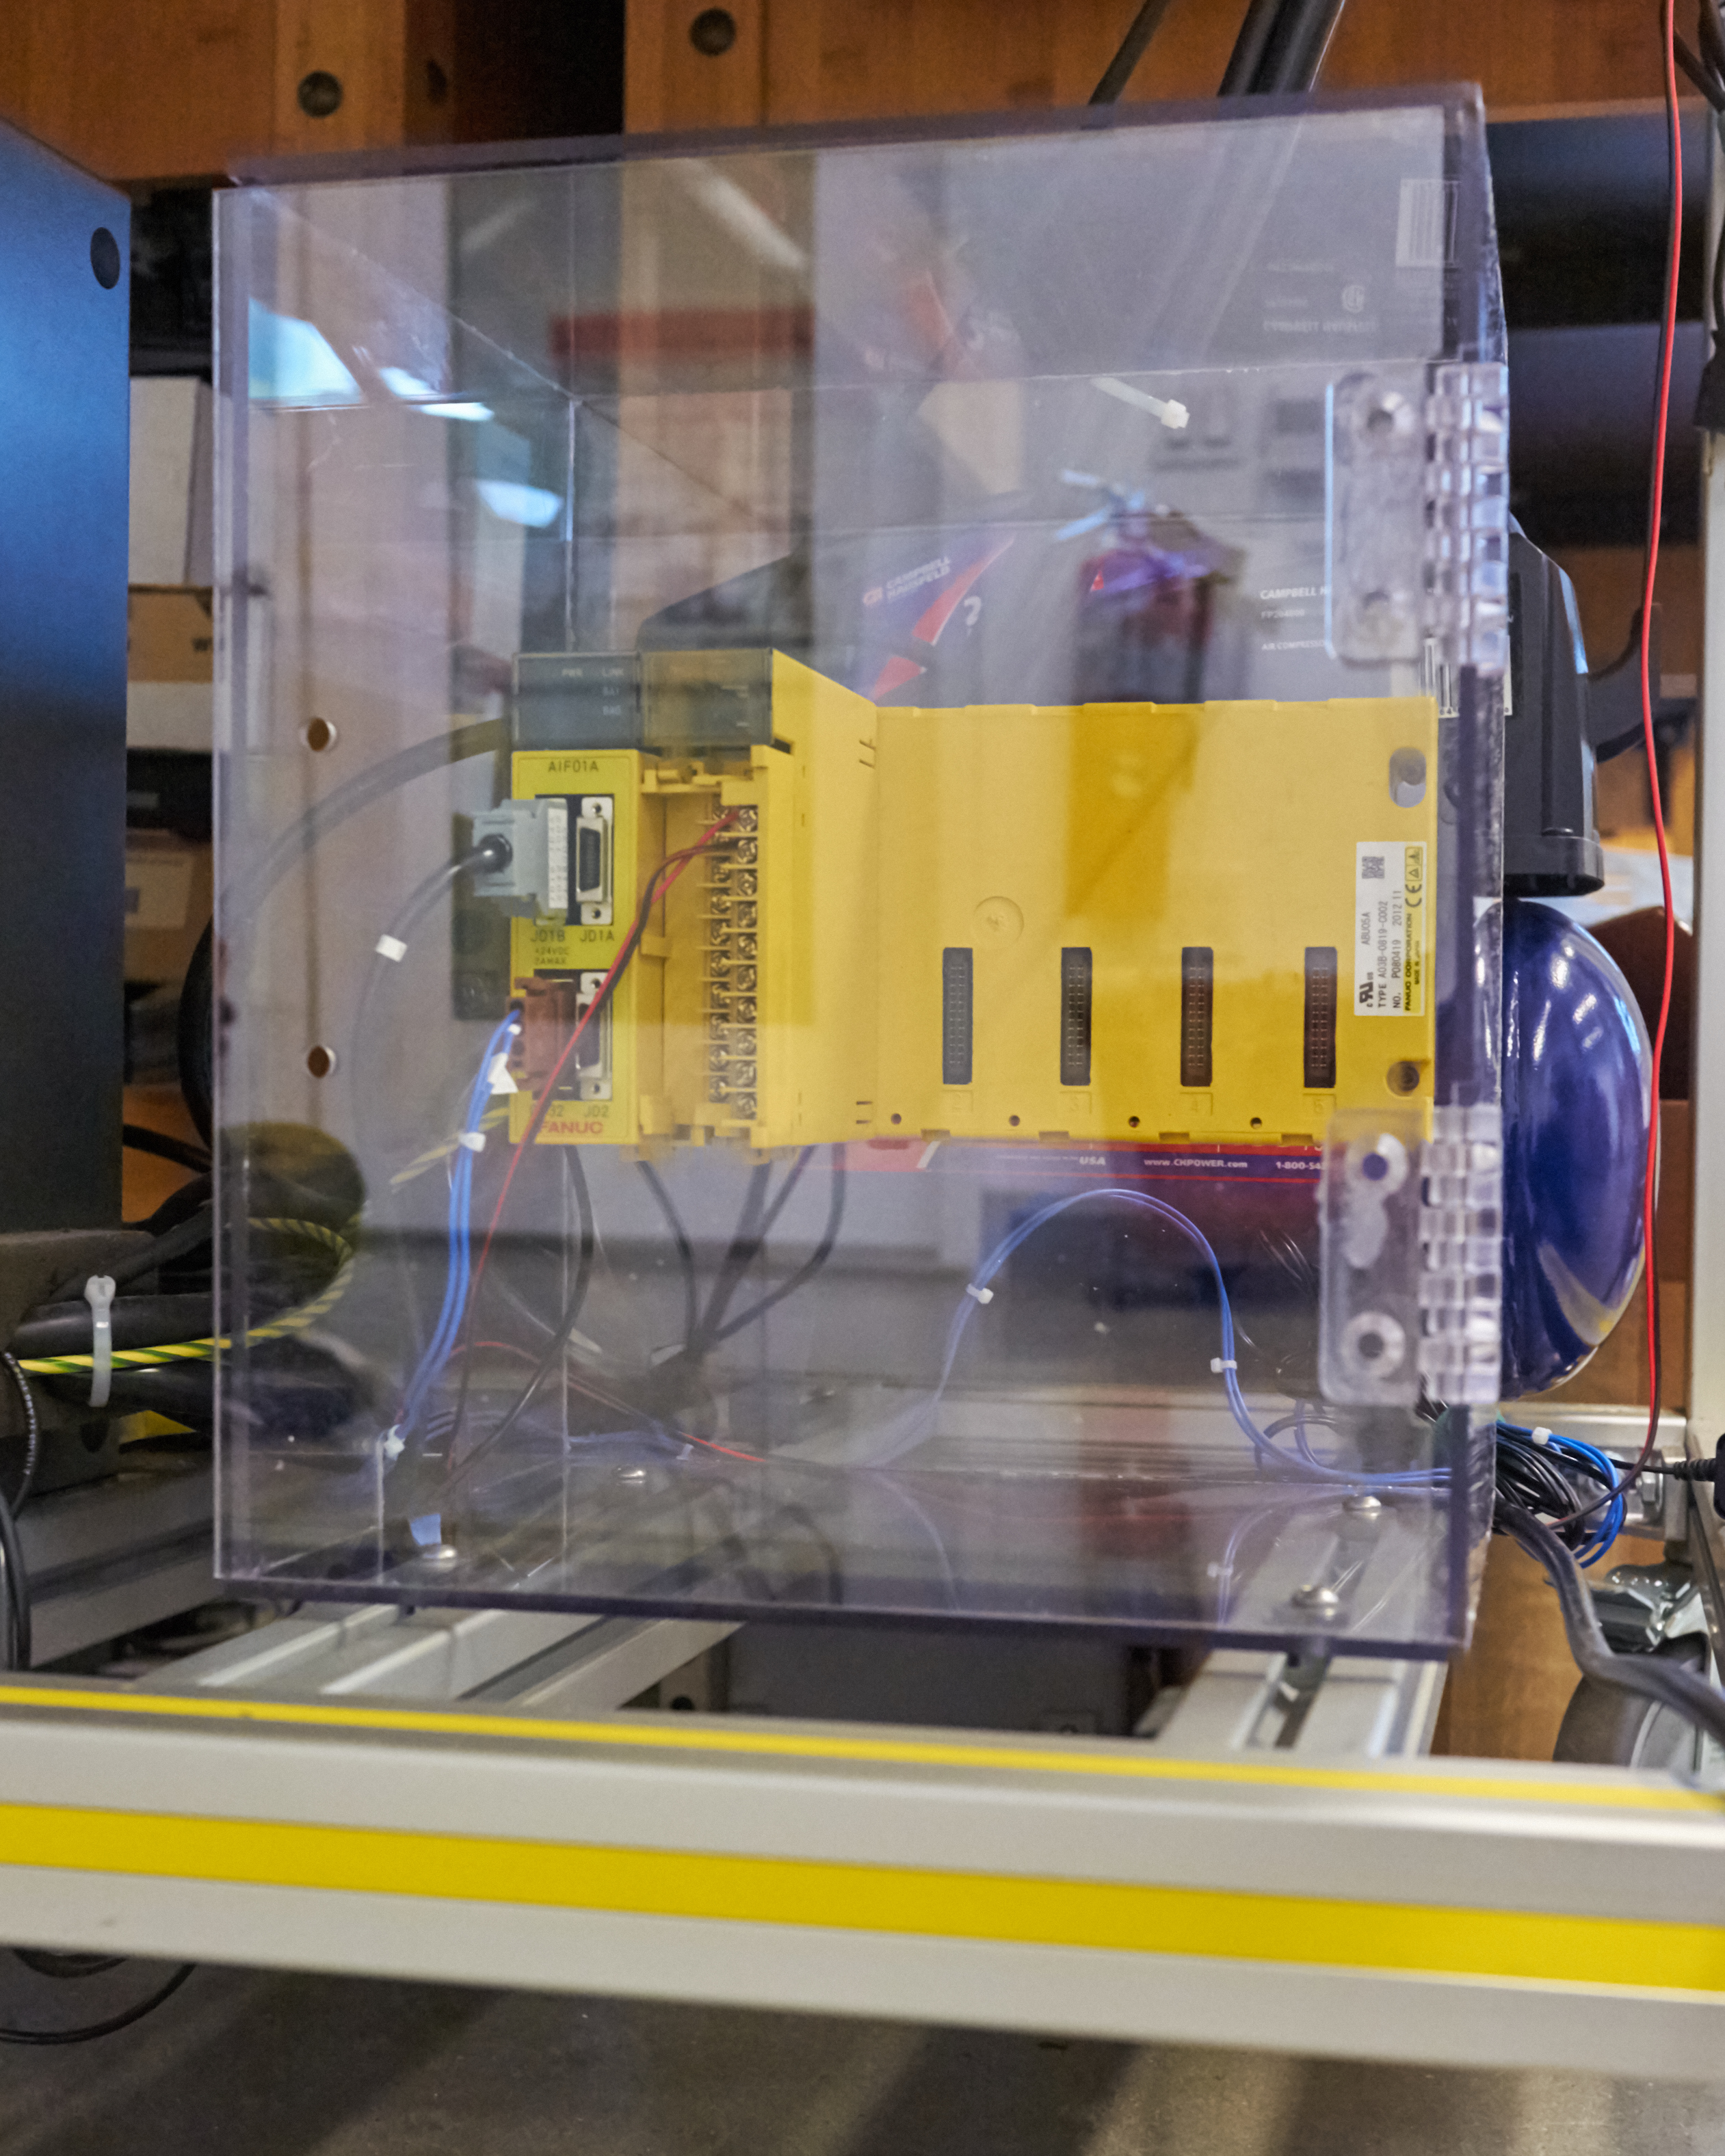
\includegraphics[width=.5\linewidth]{figures/cabinet1}
    \caption{The I/O cabinet.}
    \label{fig:cabinet-1}
    \end{figure}

\begin{figure}
    \centering
    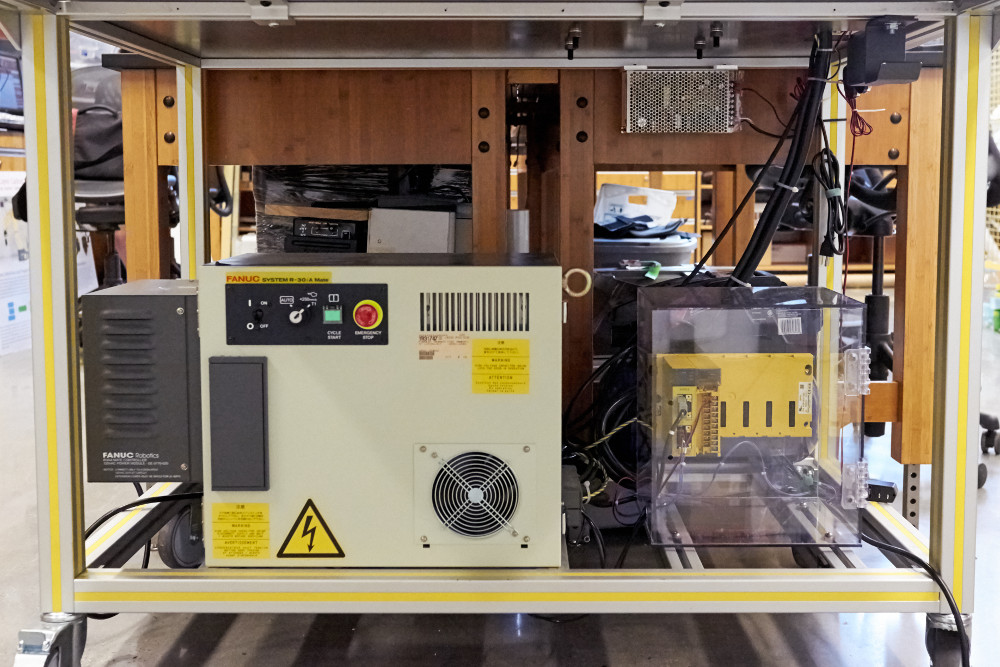
\includegraphics[width=.8\linewidth]{figures/cabinet2}
    \caption{The I/O cabinet installed alongside the FANUC controller.}
    \label{fig:cabinet-2}
\end{figure}

\begin{figure}
    \centering
    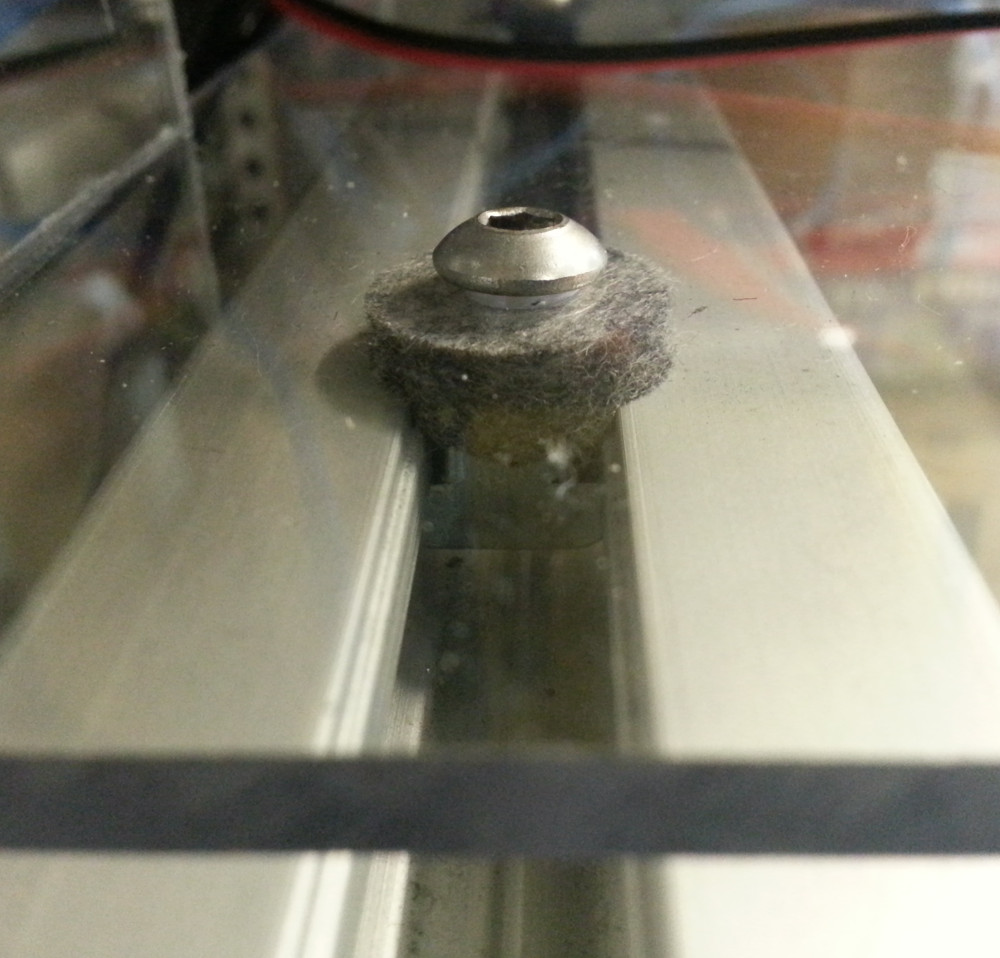
\includegraphics[width=.8\linewidth]{figures/felt-washer}
    \caption{A felt washer in the I/O cabinet mount.}
    \label{fig:felt-washer}
\end{figure}

\subsection{Megatronics board}
The Megatronics\footnote{\url{http://reprap.org/wiki/Megatronics_2.0}} board is a microcontroller board designed to drive RepRap open-source 3D printers. The board itself is based on other open-source projects, namely the Arduino Mega 2560\footnote{\url{http://www.arduino.cc/en/Main/arduinoBoardMega2560}} and the RAMPS\footnote{\url{http://reprap.org/wiki/RAMPS}} electronics design. The core features of the board are the ATmega 2560\footnote{\url{http://www.atmel.com/devices/atmega2560.aspx}} microcontroller, the Pololu stepper driver\footnote{\url{https://www.pololu.com/category/120/stepper-motor-drivers}} slots, and the extruder signal pins. The board is also set up for optional dual extruders, a heated bed, and an LCD display among other additional features. The Megatronics board was chosen for this project mostly out of convenience: although few of the board's features are used here, its compatibility with exsisting firmwares and control modules made the setup relatively easy compared to making a custom pared-down controller board. A datasheet for the board is available in Appendix~\ref{sec:mega-datasheet}.

\subsubsection{Mounting}
The Megatronics board is mounted to the frame of the CERT robot cart such that the board is accessible for modifications and the wires reach the extruder readily. The mount location also facilitates USB connection to a laptop for uploading new firmware\footnote{A 16ft USB cable was initially used in hopes of routing the cable through the frame for easy access in case the board was moved to a less accessible location. The resulting avrdude sync errors prevented any programs from uploading properly even though the cable was shorter than the recommended 5m maximum. Using a 2ft cable alleviated the problem.}. The mounted board is shown in Figure~\ref{fig:mounted-mega}. Drawings and a bill of materials for the mount are available in Appendix~\ref{sec:mega-drawings}.

\begin{figure}
    \centering
    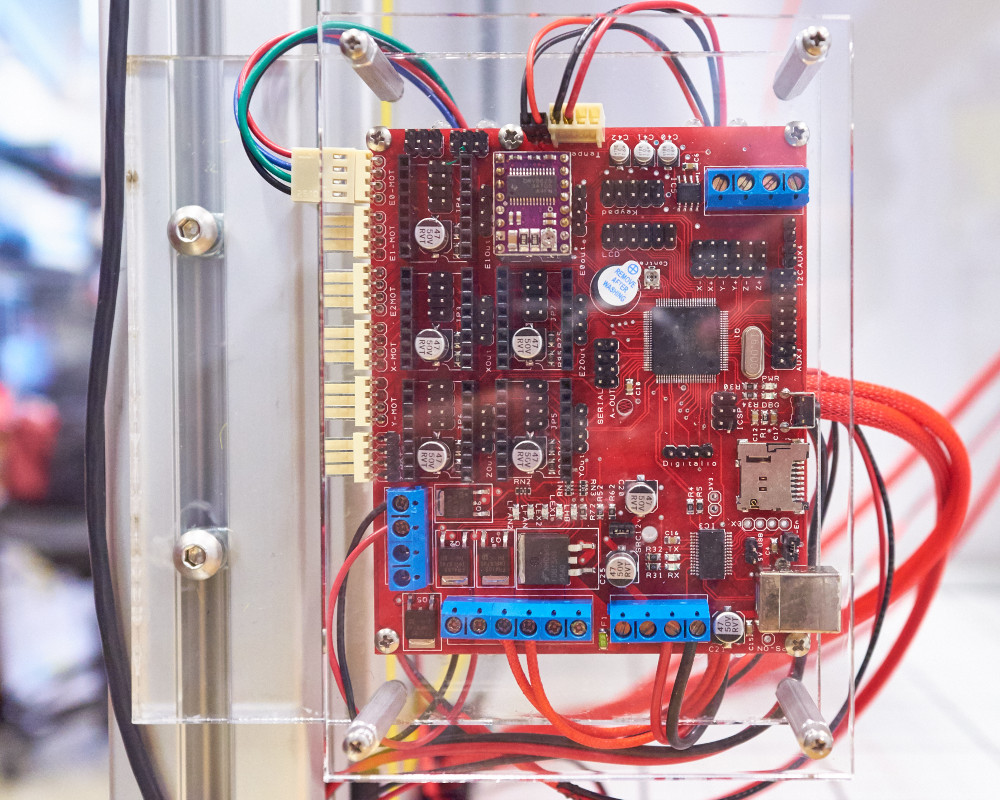
\includegraphics[width=.8\linewidth]{figures/mounted-mega}
    \caption{The mounted Megatronics board.}
    \label{fig:mounted-mega}
\end{figure}

\subsubsection{Wiring and connections}
In order to keep the wires neat where they met the board, the acrylic mount was designed with cable-tie slots, and the extruder wires were bundled in expandable polyester sleeving. These are shown in Figure~\ref{fig:mega-back}. The power and analog input wires to the board both terminate somewhere in the bottom portion of the cart, so those wires were routed through the slots in the cart's auminum extrusions, shown in Figure~\ref{fig:frame-wire-route}.

\begin{figure}
    \centering
    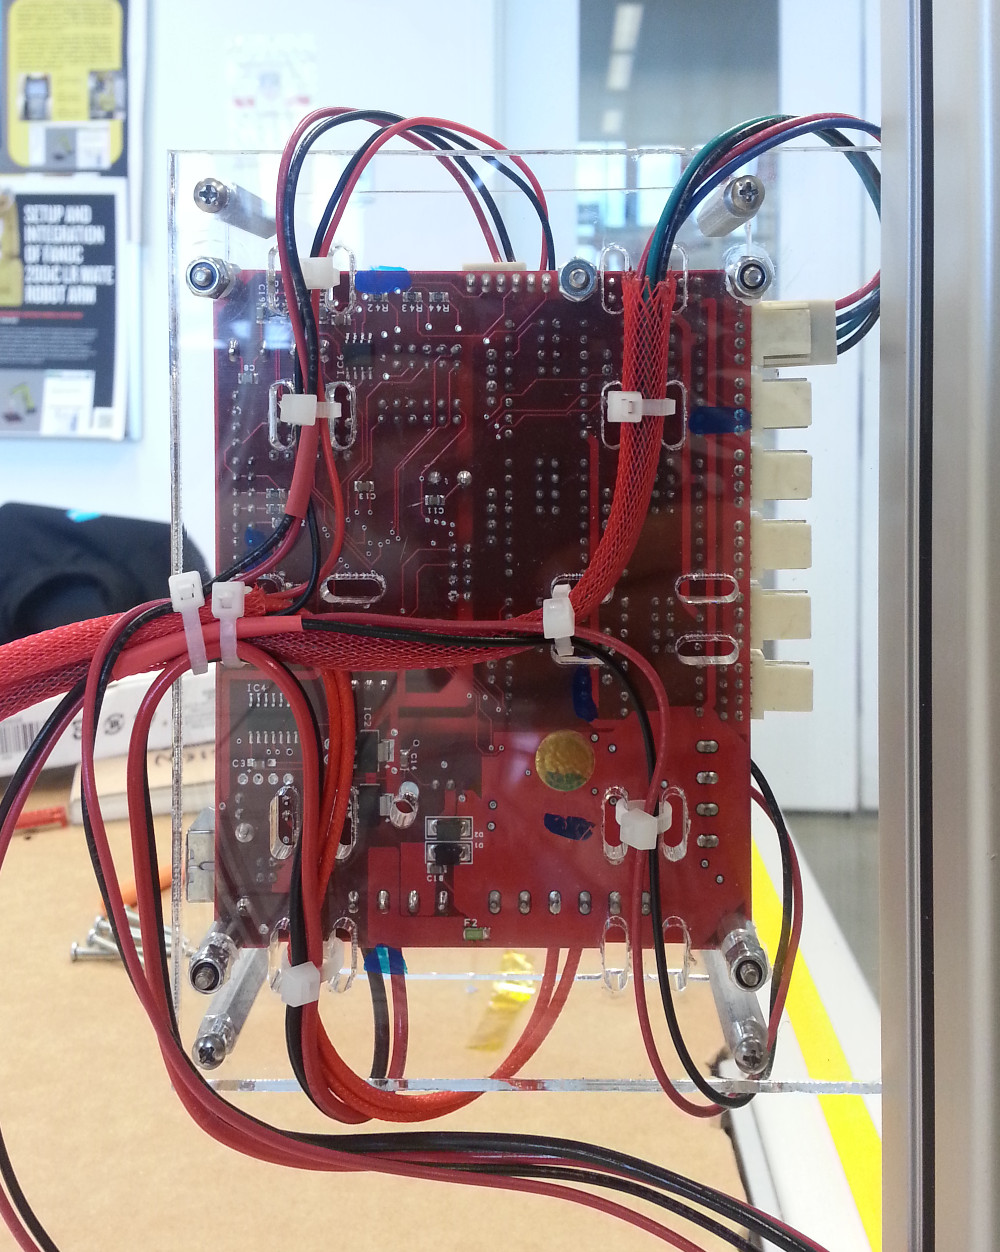
\includegraphics[width=.5\linewidth]{figures/megatronics-back}
    \caption{Wire managament at the Megatronics board.}
    \label{fig:mega-back}
\end{figure}

\begin{figure}
    \centering
    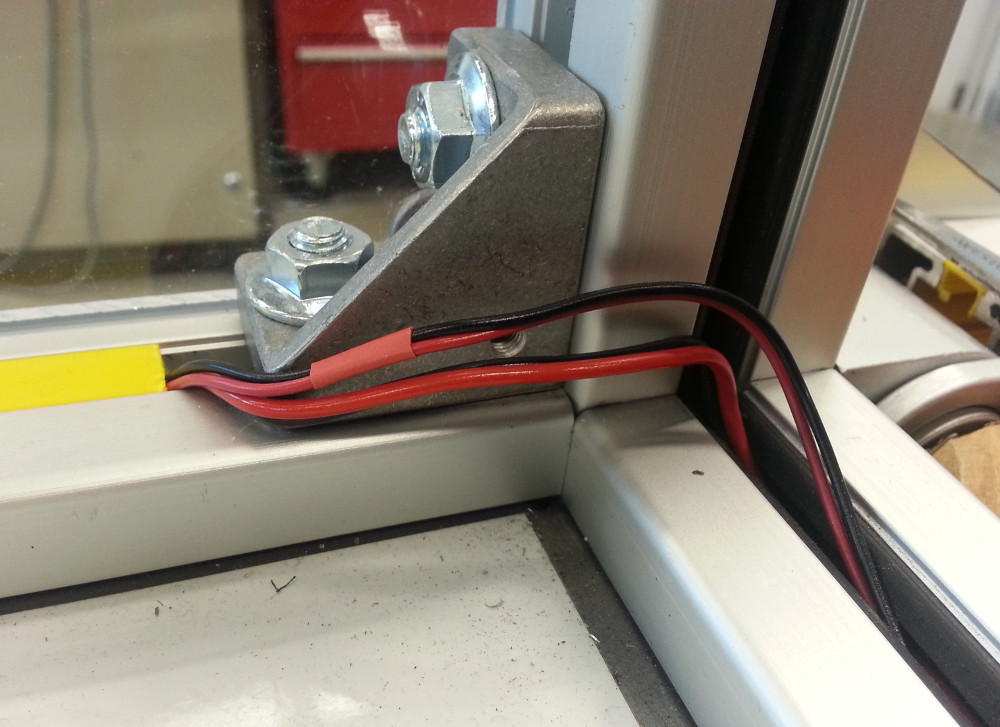
\includegraphics[width=.8\linewidth]{figures/frame-wire-route}
    \caption{Wires routed through the cart frame slots.}
    \label{fig:frame-wire-route}
\end{figure}

\subsubsection{Firmware}
The Megatronics board is compatible with the Marlin open-source 3D printer firmware. The board is generally supplied with the Marlin firmware already uploaded, but the board is open to modified or completely different firmwares in case of other development projects. The Marlin firmware exists as a Git repository hosted on Github\footnote{\url{https://github.com/}}. See Appendix~\ref{sec:more-info} for more information on Git.

Before attempting to use the full Marlin firmware, the board was tested for basic functionality using the supplied test firmware\footnote{\url{http://reprap.org/wiki/Megatronics_2.0\#Files}}. Once the board functionality was confirmed, the Marlin firmware was forked\footnote{\url{https://help.github.com/articles/fork-a-repo/}} and configured\footnote{\url{http://reprap.org/wiki/Marlin\#Configuring_and_compilation}} for this project's custom extruder. The new repository is linked in Appendix~\ref{sec:more-info}. Note in \verb|Configuration.h| that the extruder \verb|e_steps_per_mm| is calculated from on the stepper motor, gear ratio, and effective filament drive diameter of the custom extruder. Also note that \verb|FAN_PIN| and \verb|FAN2_PIN| are swapped because the Megatronics board is (for reasons unknown) missing screws from the screw terminals for Fan 1.

\subsubsection{Software}
Once the Megatronics board is set up, it is ready to take commands from a computer. It accepts G-code\footnote{\url{http://en.wikipedia.org/wiki/G-code}}, in this case, over a USB interface. G-code for RepRap 3D printers usually includes extruder motion commands, speed settings, heater temperature settings, fan speeds, and more. Usually, a 3D printed part starts as a 3D model file such as an \verb|.stl| or a \verb|.step|. A piece of computer software "slices" the model, creating the toolpath necessary to print the file. The software also uses information about the 3D printer's geometry and printing hardware to generate the appropriate G-code. Later, the computer sends the G-code to the 3D printer controller, the Megatronics board in this case, which then interprets the G-code and creates the printed part.

For this project, there is not yet any software that handles curved-layer FDM 3D printing. Thus, the "slicer" portion of the software will not be used yet. Because the extruder motion control is all handled by the FANUC robot, for now, all that is needed is a G-code sending application to control the extruder heating, cooling, and feed. Pronterface, part of the Printrun\footnote{\url{http://reprap.org/wiki/Printrun}} package, was chosen to send G-code to the Megagronics board. Pronterface is a GUI (graphical user interface) that simplifies interfacing with RepRap printers, especially while debugging the extruder itself. 

The main Pronterface interface is shown in Figure~\ref{fig:pronterface}. At a glance, the interface allows the user to connect and disconnect from printers, change feedrates, jog the motors, and set heater setpoints in addition to providing a G-code command line.

\begin{figure}
    \centering
    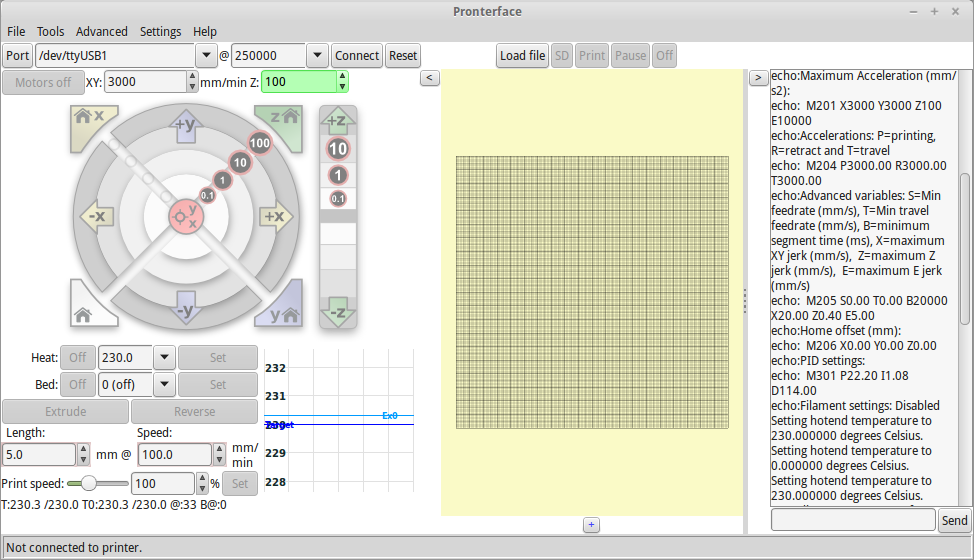
\includegraphics[width=.9\linewidth]{figures/pronterface}
    \caption{The main Pronterface interface.}
    \label{fig:pronterface}
\end{figure}

\subsection{Jameco power supply}
\subsubsection{Current requirement}
The Megatronics board can be powered from a 5V USB connection or from a 12V external power supply, as determined by on-board jumpers (see the datasheet, Appendix~\ref{sec:mega-datasheet}). The USB power from a typical laptop is adequate for communicating with and programming the board. However, driving stepper motors and heating cartridges requires far more current than a laptop USB port can supply, so a Jameco OEM power supply was chosen to power the board. The supply is rated for 11.5A at 12V. The extruder stepper motor is rated at 1.7A/phase with two phases for a total current draw of \(1.7\si{\ampere}\sqrt{2}=2.4\si{\ampere}\). The ceramic heater is rated for 30W at 12V\footnote{\url{http://www.makerfarm.com/index.php/hexagon-hot-end.html}}, for a current draw of \(\frac{30\si{\watt}}{12\si{\volt}}=2.5\si{\ampere}\). There are no other significant electrical loads in the extruder, so the Jameco power supply is adequate for the custom extruder. The power supply datasheet is available in Appendix~\ref{sec:jameco-datasheet}.

\subsubsection{Mounting}
The power supply was mounted at the rear of the underside of the CERT cart bed frame. The mounted supply is pictured in Figure~\ref{fig:jameco-mounted}. The mounting location was chosen for easy access for future wiring activities. A clear acrylic cover was made to protect any person or foreign object from accidentally touching the screw terminals. The cover was laser cut and then bent to shape using a purpose-built strip heater, shown in Figure~\ref{fig:strip-heat}. Drawings and a bill of materials for the mounting setup are available in Appendix~\ref{sec:jameco-drawings}.

\begin{figure}
    \centering
    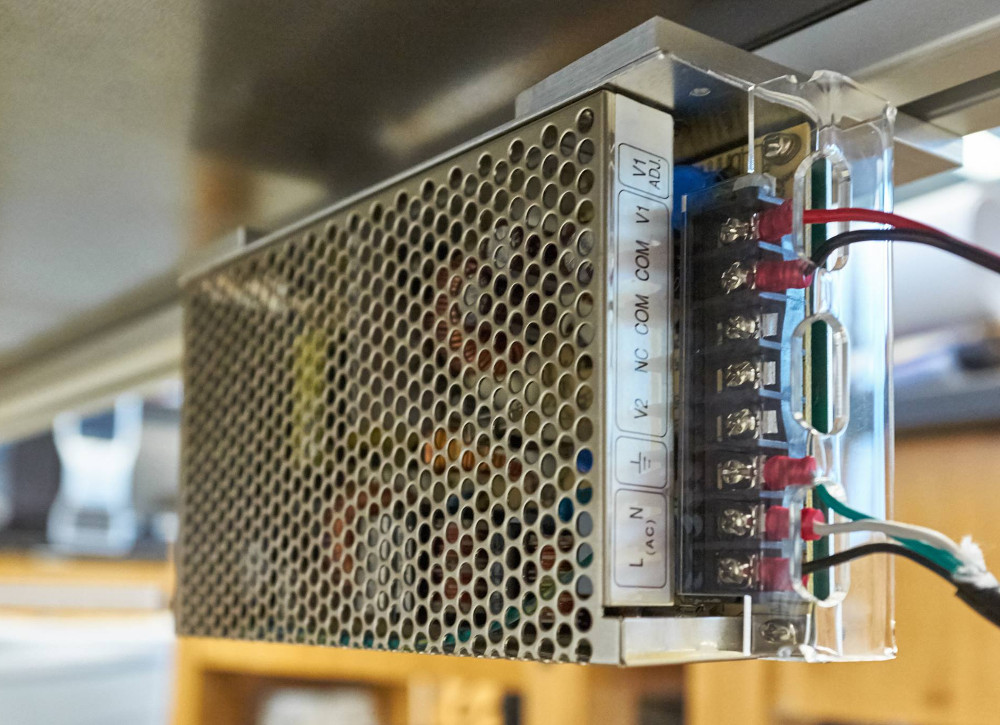
\includegraphics[width=.8\linewidth]{figures/jameco-mounted}
    \caption{The mounted Jameco power supply.}
    \label{fig:jameco-mounted}
\end{figure}

\begin{figure}
    \centering
    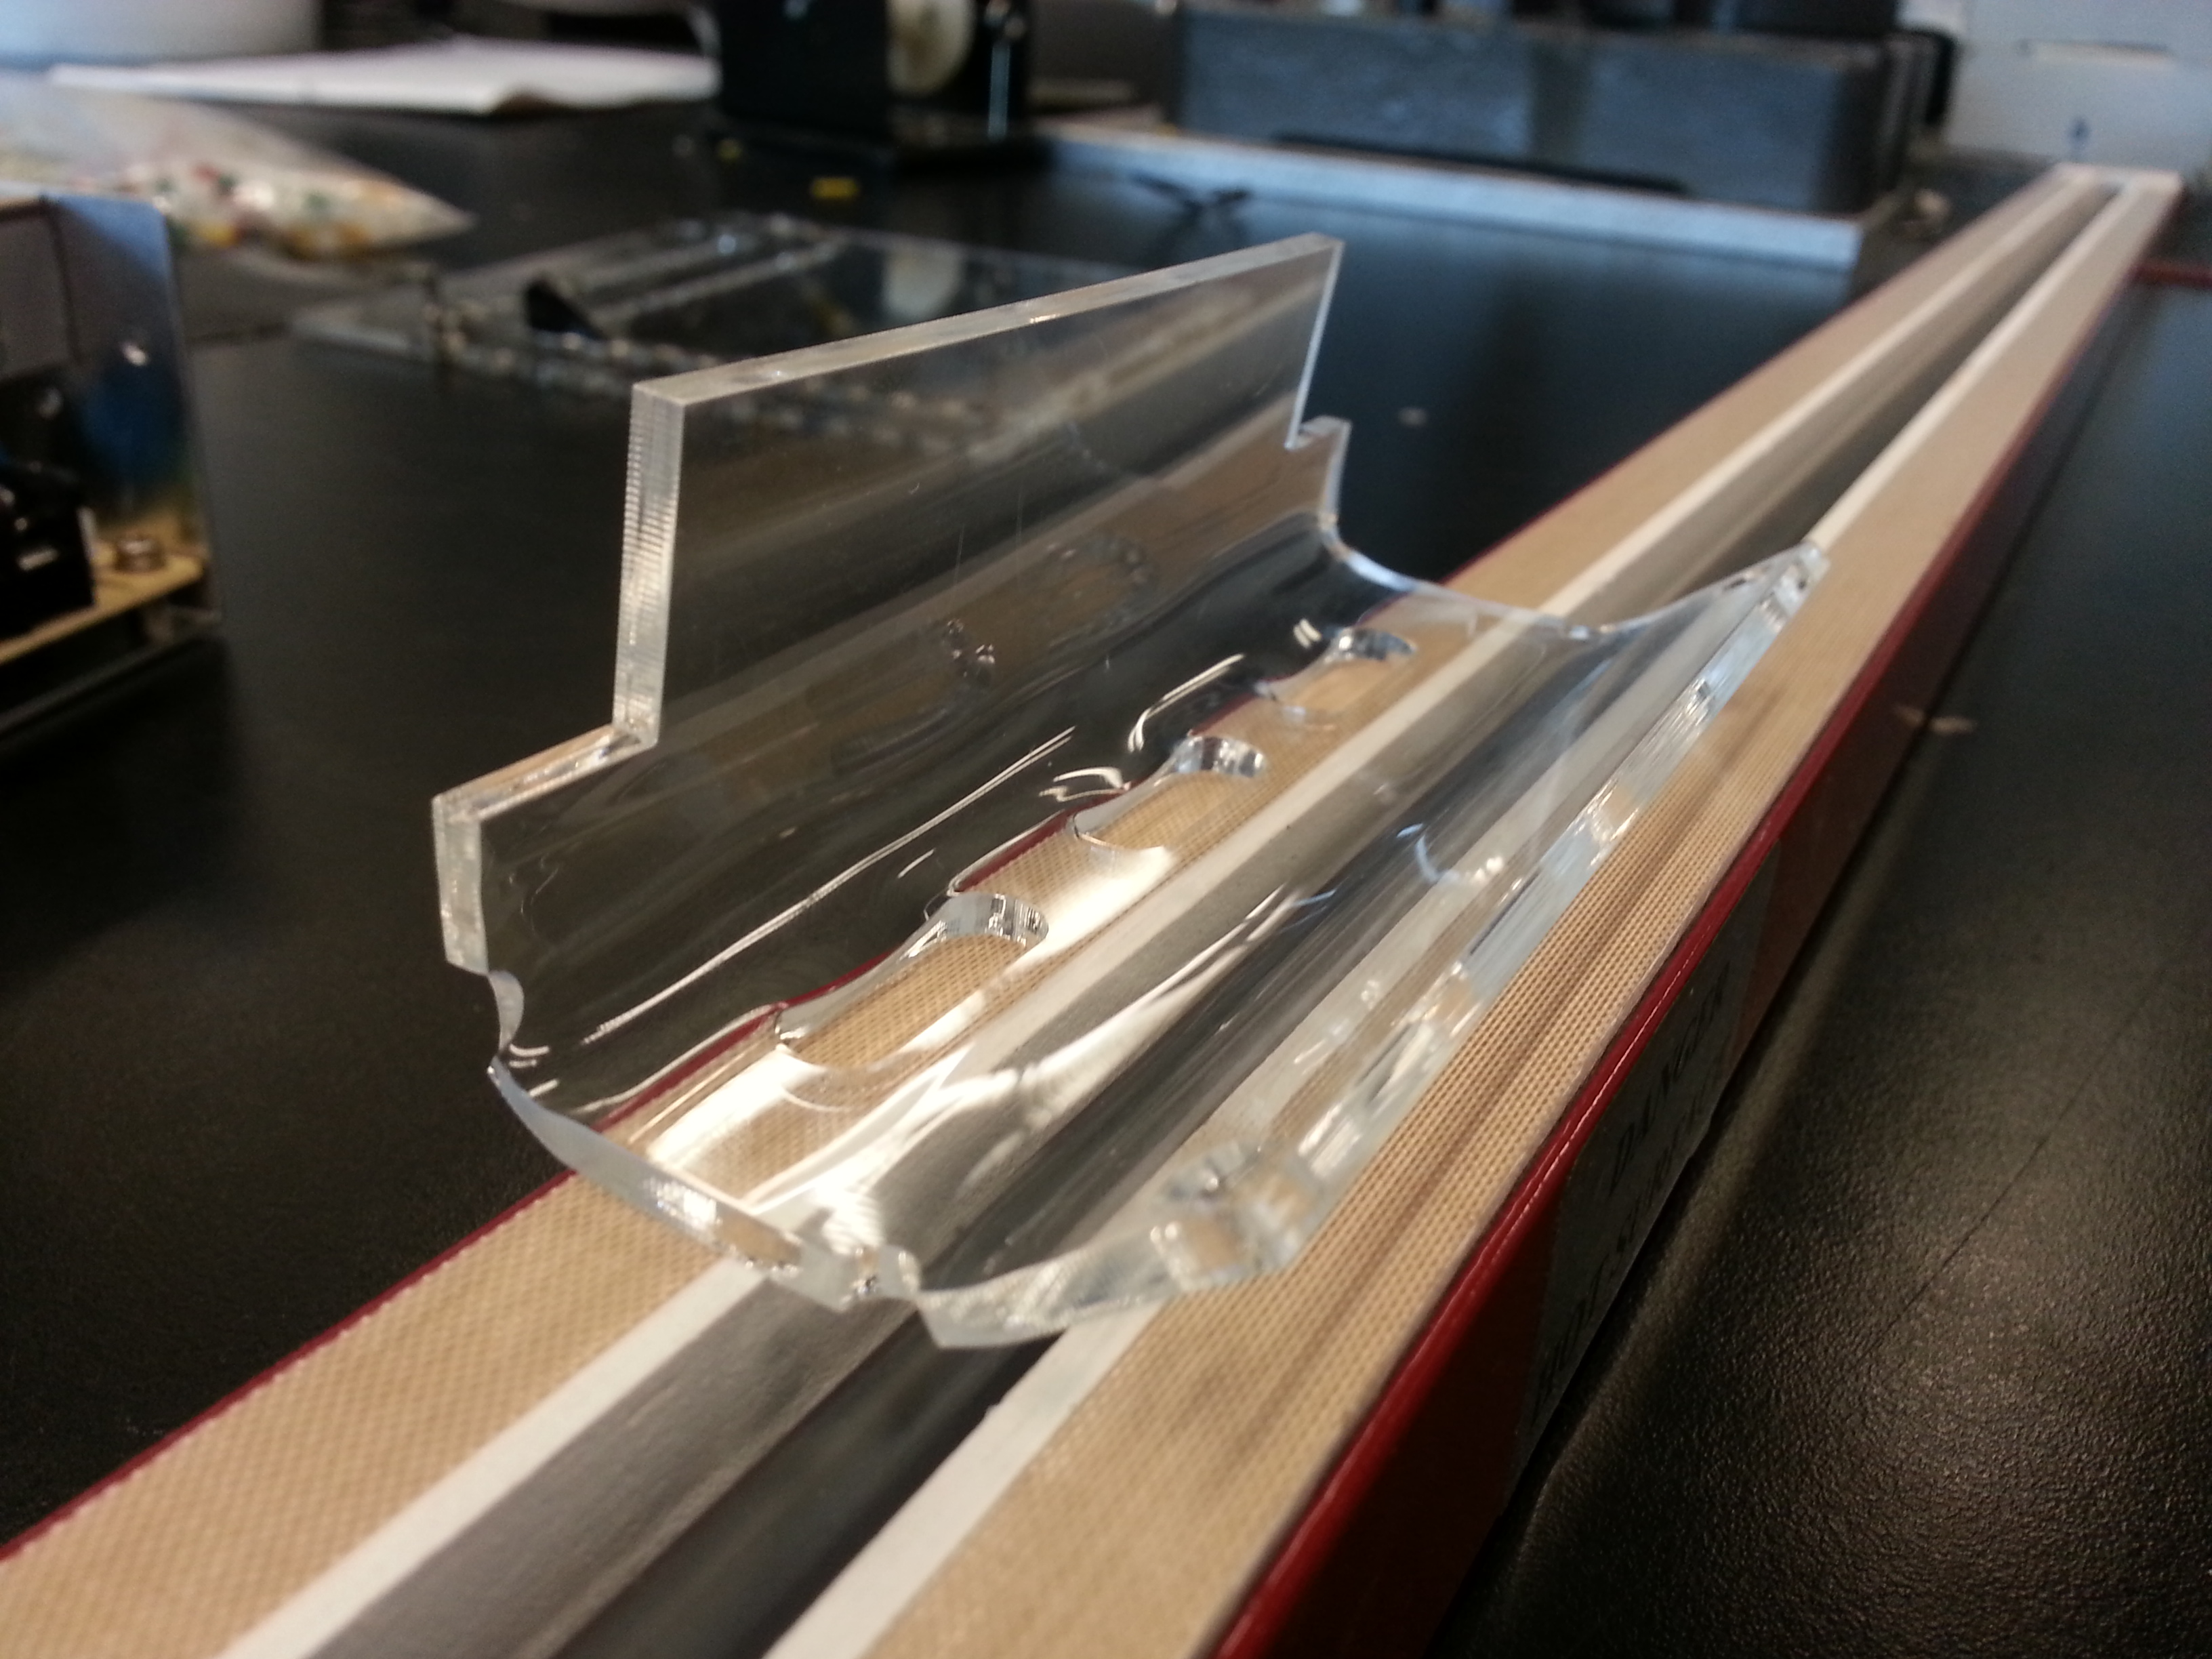
\includegraphics[width=.8\linewidth]{figures/strip-heat}
    \caption{Power supply screw terminal cover on the strip heater.}
    \label{fig:strip-heat}
\end{figure}
